\de{ĐỀ THI HỌC KỲ I NĂM HỌC 2022-2023}{TRƯỜNG THPT CHUYÊN LÊ KHIẾT - QUẢNG NGÃI}
\begin{center}
	\textbf{PHẦN 1 - TRẮC NGHIỆM}
\end{center}
\Opensolutionfile{ans}[ans/ans]

	\begin{ex}[0H1Y1-2]%[Dự án đề kiểm tra HKI NH22-23- Dương Phước Sang]%[Chuyên Lê Khiết - Quãng Ngãi]
		Biết rằng $\sin\alpha=\dfrac{\sqrt{3}}{2}$ với $90^{\circ} <\alpha<180^{\circ}$. Giá trị của $\alpha$ là bao nhiêu?
		\choice
		{$\alpha=150^{\circ}$}
		{$\alpha=60^{\circ}$}
		{$\alpha=30^{\circ}$}
		{\True $\alpha=120^{\circ}$}
		\loigiai{
			Ta có $\sin 120^{\circ}=\dfrac{\sqrt{3}}{2}$ và $90^{\circ} <120^{\circ}<180^{\circ}$ nên $\alpha=120^{\circ}$.
		}
	\end{ex}

	\begin{ex}[0H2B2-3]%[Dự án đề kiểm tra HKI NH22-23- Dương Phước Sang]%[Chuyên Lê Khiết - Quãng Ngãi]
		Cho bốn điểm bất kì $A$, $B$, $C$, $O$. Đẳng thức nào sau đây là đúng?
		\choice
		{$\overrightarrow{AB}=\overrightarrow{OB}+\overrightarrow{OA}$}
		{$\overrightarrow{OA}=\overrightarrow{OB}+\overrightarrow{AB}$}
		{$\overrightarrow{AB}=\overrightarrow{AC}+\overrightarrow{BC}$}
		{\True $\overrightarrow{OA}=\overrightarrow{OC}+\overrightarrow{CA}$}
		\loigiai{
			Đẳng thức đúng là $\overrightarrow{OA}=\overrightarrow{OC}+\overrightarrow{CA}$.
		}
	\end{ex}

	\begin{ex}[0H2B4-1]%[Dự án đề kiểm tra HKI NH22-23- Dương Phước Sang]%[Chuyên Lê Khiết - Quãng Ngãi]
		Cho tam giác $ABC$ là tam giác đều. Góc giữa hai véc-tơ $\overrightarrow{AB}$ và $\overrightarrow{BC}$ nhận giá trị nào sau đây?
		\choice
		{\True $120^{\circ}$}
		{$45^{\circ}$}
		{$30^{\circ}$}
		{$60^{\circ}$}
		\loigiai{
			\immini{Ta có $\left(\overrightarrow{AB},\overrightarrow{BC}\right)=180^{\circ} -\left(\overrightarrow{BA},\overrightarrow{BC}\right)=180^{\circ} -\widehat{ABC}=180^{\circ} -60^{\circ}=120^{\circ}$.}
			{\begin{tikzpicture}[>=stealth,line join=round,line cap=round,font=\footnotesize,scale=0.5]
					\clip(-1,-1) rectangle (7,6);
					\path 
					(0,0) coordinate (B)
					(6,0) coordinate (C)
					(B) arc (-180:120:6) coordinate (A)
					;			
					\draw 
					(A)--(B)--(C)--(A);
					\foreach \i/\g in {A/90, B/180,C/0}
					\fill (\i) circle (1.5pt)+(\g:4mm) node {$\i$};
				\end{tikzpicture}
			}
		}
	\end{ex}

	\begin{ex}[0D1Y1-1]%[Dự án đề kiểm tra HKI NH22-23- Dương Phước Sang]%[Chuyên Lê Khiết - Quãng Ngãi]
		Trong các câu sau, câu nào là mệnh đề chứa biến?
		\choice
		{\lq\lq $23$ là số nguyên tố\rq\rq}
		{\lq\lq $\sqrt{3}$ là số hữu tỉ\rq\rq}
		{\lq\lq $16$ là số chính phương\rq\rq}
		{\True \lq\lq $2x^2+3x+5=0$\rq\rq}
		\loigiai{
			Mệnh đề chứa biến là \lq\lq $2x^2+3x+5=0$\rq\rq.
		}
	\end{ex}

	\begin{ex}[0H2Y1-3]%[Dự án đề kiểm tra HKI NH22-23- Dương Phước Sang]%[Chuyên Lê Khiết - Quãng Ngãi]
		Cho hình bình hành $ABCD$, gọi $O$ là giao điểm của $AC$ và $BD$. Đẳng thức nào sau đây là đẳng thức {\bf sai}?
		\choice
		{\True $\overrightarrow{OA}=\overrightarrow{OC}$}
		{$\overrightarrow{BC}=\overrightarrow{AD}$}
		{$\overrightarrow{OB}=\overrightarrow{DO}$}
		{$\overrightarrow{AB}=\overrightarrow{DC}$}
		\loigiai{
			\immini{Đẳng thức sai là $\overrightarrow{OA}=\overrightarrow{OC}$ vì $\overrightarrow{OA}$ và $\overrightarrow{OC}$ ngược hướng.}
			{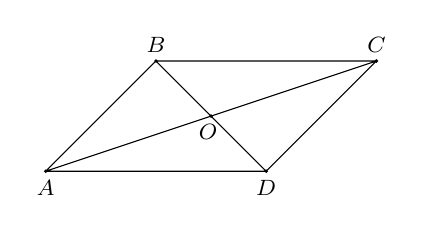
\begin{tikzpicture}[scale=0.7, font=\footnotesize, line join=round, line cap=round,>=stealth]
					\path 
					(0,0) coordinate (A)
					(6,2) coordinate (C)
					(2,2) coordinate (B) 
					(4,0) coordinate (D) 
					(3,1) coordinate (O) 
					;
					\draw (A)--(B)--(C)--(D)--(A)--(C) (B)--(D);
					\foreach \x/\g in {A/-90,B/90,C/90,D/-90,O/-100} 
					\fill[black] (\x) circle (1pt)+(\g:3mm) node {$\x$};
			\end{tikzpicture}}
		}
	\end{ex}

	\begin{ex}[0H3B1-4]%[Dự án đề kiểm tra HKI NH22-23- Dương Phước Sang]%[Chuyên Lê Khiết - Quãng Ngãi]
		Trong mặt phẳng tọa độ $Oxy$, véc-tơ nào sau đây cùng phương với $\overrightarrow{a}=\left(\dfrac{1}{3};-1\right)$?
		\choice
		{$\overrightarrow{u_1}=\left(\dfrac{1}{3};1\right)$}
		{$\overrightarrow{u_4}=\left(2;6\right)$}
		{\True $\overrightarrow{u_3}=\left(-2;6\right)$}
		{$\overrightarrow{u_2}=\left(1;-\dfrac{1}{3}\right)$}
		\loigiai{
			Ta có $\dfrac{\frac{1}{3}}{-2}=\dfrac{-1}{6}$ nên $\overrightarrow{a}$ cùng phương với $\overrightarrow{u_3}=\left(-2;6\right)$.
		}
	\end{ex}

	\begin{ex}[0H3Y2-1]%[Dự án đề kiểm tra HKI NH22-23- Dương Phước Sang]%[Chuyên Lê Khiết - Quãng Ngãi]
		Cho $\overrightarrow{u}=(-2;2)$ và $\overrightarrow{v}=(4;-2)$. Tích vô hướng của $\overrightarrow{u}$ và $\overrightarrow{v}$ là
		\choice
		{\True $-12$}
		{$-8$}
		{$2$}
		{$10$}
		\loigiai{
			Ta có $\overrightarrow{u}\cdot\overrightarrow{v}=-2\cdot 4+2\cdot (-2)=-12$.
		}
	\end{ex}

	\begin{ex}[0H2Y3-1]%[Dự án đề kiểm tra HKI NH22-23- Dương Phước Sang]%[Chuyên Lê Khiết - Quãng Ngãi]
		Đẳng thức nào sau đây mô tả đúng hình vẽ sau
		\begin{center}
			\begin{tikzpicture}[scale=1, font=\footnotesize, line join=round, line cap=round,>=stealth]
				\path 
				(0,0) coordinate (I) 
				(2,0) coordinate (A)
				(4,0) coordinate (C) 
				(6,0) coordinate (D) 
				(8,0) coordinate (B) 
				;
				\draw (I)--(B);
				\foreach \x/\g in {A/-90,B/0,I/180} 
				\fill[black] (\x) circle (2pt)+(\g:3mm) node {$\x$};
				\foreach \x in {C,D} 
				\fill[black] (\x) circle (2pt);
			\end{tikzpicture}
		\end{center}
		\choice
		{\True $\overrightarrow{AB}=-3\overrightarrow{AI}$}
		{$\overrightarrow{AI}=\dfrac{1}{3}\overrightarrow{AB}$}
		{$\overrightarrow{AB}=3\overrightarrow{AI}$}
		{$\overrightarrow{AB}=-3\overrightarrow{IA}$}
		\loigiai{
			Ta có $\heva{&AB=3AI\\ &\overrightarrow{AB}, \overrightarrow{AI} \text{ ngược hướng}}$ nên $\overrightarrow{AB}=-3\overrightarrow{AI}$.
		}
	\end{ex}

	\begin{ex}[0D1Y1-4]%[Dự án đề kiểm tra HKI NH22-23- Dương Phước Sang]%[Chuyên Lê Khiết - Quãng Ngãi]
		Viết số quy tròn của $\pi$ đến hàng phần nghìn.
		\choice
		{$3{,}14$}
		{\True $3{,}142$}
		{$3{,}141$}
		{$3{,}1416$}
		\loigiai{
			Số quy tròn của $\pi$ đến hàng phần nghìn là $3{,}142$.
		}
	\end{ex}

	\begin{ex}[0H3Y1-3]%[Dự án đề kiểm tra HKI NH22-23- Dương Phước Sang]%[Chuyên Lê Khiết - Quãng Ngãi]
		Trong mặt phẳng tọa độ $Oxy$, cho véc-tơ $\overrightarrow{u}=2\overrightarrow{i}-3\overrightarrow{j}$. Tọa độ của $\overrightarrow{u}$ là
		\choice
		{\True $(2;-3)$}
		{$(-2;3)$}
		{$(-3;2)$}
		{$(2;3)$}
		\loigiai{
			Tọa độ của $\overrightarrow{u}=2\overrightarrow{i}-3\overrightarrow{j}$ là $(2;-3)$.
		}
	\end{ex}

	\begin{ex}[0H1Y2-2]%[Dự án đề kiểm tra HKI NH22-23- Dương Phước Sang]%[Chuyên Lê Khiết - Quãng Ngãi]
		Cho tam giác $ABC$ với các cạnh $AB=c$, $BC=a$, $CA=b$. Gọi $S$ là diện tích của tam giác $ABC$. Trong các phát biểu sau, phát biểu nào là đúng?
		\choice
		{\True $S=\dfrac{1}{2}bc\sin A$}
		{$S=\dfrac{1}{2}bc\sin B$}
		{$S=\dfrac{1}{2}ab\sin A$}
		{$S=\dfrac{1}{2}ac\sin A$}
		\loigiai{
			Diện tích của tam giác là $S=\dfrac{1}{2}bc\sin A$.
		}
	\end{ex}

	\begin{ex}[0D2Y1-1]%[Dự án đề kiểm tra HKI NH22-23- Dương Phước Sang]%[Chuyên Lê Khiết - Quãng Ngãi]
		Bất phương trình nào sau đây là bất phương trình bậc nhất hai ẩn?
		\choice
		{$2x^2+3x+1>0$}
		{\True $2x+y>5$}
		{$2x^2+5y^2>3$}
		{$2x+5y-3z>0$}
		\loigiai{
			Bất phương trình $2x+y>5$ là bất phương trình bậc nhất hai ẩn.
		}
	\end{ex}

	\begin{ex}[0D2Y2-1]%[Dự án đề kiểm tra HKI NH22-23- Dương Phước Sang]%[Chuyên Lê Khiết - Quãng Ngãi]
		Trong các cặp số $(x;y)$ sau, cặp nào là nghiệm của hệ bất phương trình $\heva{&2x>y-1\\&x+2y\leq 3.}$
		\choice
		{$(1;2)$}
		{\True $(1;0)$}
		{$(1;3)$}
		{$(1;4)$}
		\loigiai{
			\begin{itemize}
				\item Thế $x=1$, $y=2$ vào bất phương trình ta được $\heva{&2\cdot 1>2-1\\ &1+2\cdot 2\leq 3}$ là kết quả sai.\\
				Vậy $(1;2)$ không là nghiệm của hệ bất phương trình.
				\item Thế $x=1$, $y=0$ vào bất phương trình ta được $\heva{&2\cdot 1>0-1\\ &1+2\cdot 0\leq 3}$ là kết quả đúng.\\
				Vậy $(1;0)$ là nghiệm của hệ bất phương trình.
				\item Thế $x=1$, $y=3$ vào bất phương trình ta được $\heva{&2\cdot 1>3-1\\ &1+2\cdot 3\leq 3}$ là kết quả sai.\\
				Vậy $(1;3)$ không là nghiệm của hệ bất phương trình.
				\item Thế $x=1$, $y=4$ vào bất phương trình ta được $\heva{&2\cdot 1>4-1\\ &1+2\cdot 4\leq 3}$ là kết quả sai.\\
				Vậy $(1;4)$ không là nghiệm của hệ bất phương trình.
			\end{itemize}
		}
	\end{ex}

	\begin{ex}[0H2Y3-1]%[Dự án đề kiểm tra HKI NH22-23- Dương Phước Sang]%[Chuyên Lê Khiết - Quãng Ngãi]
		Cho $\overrightarrow{a}=k\overrightarrow{b}$. Đẳng thức véc-tơ nào sau đây đúng?
		\choice 
		{$\overrightarrow{a}=\left|k\right|\overrightarrow{b}$}
		{$\left|\overrightarrow{a}\right|=-k\left|\overrightarrow{b}\right|$}
		{\True $\left|\overrightarrow{a}\right|=\left|k\right| \left|\overrightarrow{b}\right|$}
		{$\left|\overrightarrow{a}\right|=k\left|\overrightarrow{b}\right|$}
		\loigiai{
			Đẳng thức véc-tơ đúng là $\left|\overrightarrow{a}\right|=\left|k\right| \left|\overrightarrow{b}\right|$.
		}
	\end{ex}

	\begin{ex}[0H1Y1-3]%[Dự án đề kiểm tra HKI NH22-23- Dương Phước Sang]%[Chuyên Lê Khiết - Quãng Ngãi]
		Trong các đẳng thức sau, đẳng thức nào là đúng?
		\choice
		{$\sin\left(180^{\circ} -\alpha\right)=-\cos\alpha$}
		{$\sin\left(180^{\circ} -\alpha\right)=\cos\alpha$}
		{$\sin\left(180^{\circ} -\alpha\right)=-\sin\alpha$}
		{\True $\sin\left(180^{\circ} -\alpha\right)=\sin\alpha$}
		\loigiai{
			Đẳng thức đúng là $\sin\left(180^{\circ} -\alpha\right)=\sin\alpha$.
		}
	\end{ex}

	\begin{ex}[0H3B2-3]%[Dự án đề kiểm tra HKI NH22-23- Dương Phước Sang]%[Chuyên Lê Khiết - Quãng Ngãi]
		Trong mặt phẳng tọa độ $Oxy$, cho các điểm $M(-5;10)$ và $N(-4;3)$. Độ dài của véc-tơ $\overrightarrow{MN}$ là
		\choice
		{$4\sqrt{3}$}
		{\True $5\sqrt{2}$}
		{$2\sqrt{22}$}
		{$5\sqrt{10}$}
		\loigiai{
			Ta có $MN=\sqrt{(-4+5)^2+(3-10)^2}=5\sqrt{2}$.
		}
	\end{ex}

	\begin{ex}[0D1B2-2]%[Dự án đề kiểm tra HKI NH22-23- Dương Phước Sang]%[Chuyên Lê Khiết - Quãng Ngãi]
		Cho ba tập hợp $A=\left\lbrace 0;1;2;3;4;5;6;7\right\rbrace$, $B=\left\lbrace 0;2;4;6;8\right\rbrace$, $C=\left\lbrace 1;3;5;7\right\rbrace$. Khẳng định nào sau đây là đúng?
		\choice
		{\True $C\subset A$}
		{$B\subset A$}
		{$A\subset B$}
		{$A\subset C$}
		\loigiai{
			Khẳng định đúng là $C\subset A$.
		}
	\end{ex}

	\begin{ex}[0H2Y1-2]%[Dự án đề kiểm tra HKI NH22-23- Dương Phước Sang]%[Chuyên Lê Khiết - Quãng Ngãi]
		Cho hình bình hành $ABCD$. véc-tơ nào sau đây cùng phương với $\overrightarrow{DC}$?
		\choice
		{\True $\overrightarrow{BA}$, $\overrightarrow{CD}$, $\overrightarrow{AB}$}
		{$\overrightarrow{BA}$, $\overrightarrow{CD}$, $\overrightarrow{CB}$}
		{$\overrightarrow{BC}$, $\overrightarrow{CD}$, $\overrightarrow{DA}$}
		{$\overrightarrow{AD}$, $\overrightarrow{CD}$, $\overrightarrow{DC}$}
		\loigiai{
			\immini{Ta có véc-tơ cùng phương với $\overrightarrow{DC}$ là $\overrightarrow{BA}$, $\overrightarrow{CD}$, $\overrightarrow{AB}$.}
			{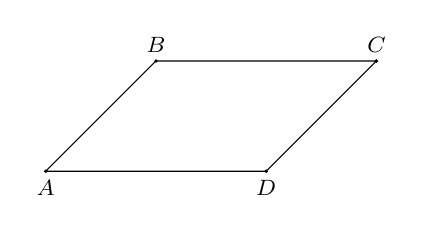
\begin{tikzpicture}[scale=0.7, font=\footnotesize, line join=round, line cap=round,>=stealth]
					\path 
					(0,0) coordinate (A)
					(6,2) coordinate (C)
					(2,2) coordinate (B) 
					(4,0) coordinate (D) 
					;
					\draw (A)--(B)--(C)--(D)--(A);
					\foreach \x/\g in {A/-90,B/90,C/90,D/-90} 
					\fill[black] (\x) circle (1pt)+(\g:3mm) node {$\x$};
			\end{tikzpicture}}
		}
	\end{ex}
	
%Câu19
\begin{ex}%[0X1Y1-1]%[Dự án đề kiểm tra HKII NH22-23- Phan Trung Hiếu]%[THPT Chuyên Lê Khiết - Quãng Ngãi]
	Một kết quả đo chiều dài của cây thuớc được ghi là $40\pm0{,}2$ (cm). Sai số tương đối của phép đo chiều dài cây thước là
	\choice
	{$\Delta\leq0{,}2$}
	{$\delta=\dfrac{2}{10}$}
	{$\Delta=0{,}2$}
	{\True $\delta\leq\dfrac{1}{200}$}
	\loigiai{
		Sai số tương đối phép đo chiều dài cây thuớc là $\delta\leq\dfrac{0{,}2}{40}=\dfrac{1}{200}$.
	}
\end{ex}
%Câu20
\begin{ex}%[0H2Y2-3]%[Dự án đề kiểm tra HKII NH22-23- Phan Trung Hiếu]%[THPT Chuyên Lê Khiết - Quãng Ngãi]
	Cho hình bình hành $ABCD$. Đẳng thức nào sau đây đúng?
	\choice
	{$\vv{AB}+\vv{BC}=\vv{BD}$}
	{$\vv{AB}+\vv{DB}=\vv{AC}$}
	{$\vv{BA}+\vv{BC}=\vv{DB}$}
	{\True$\vv{AB}+\vv{AD}=\vv{AC}$}
	\loigiai{
		Theo quy tắc hình bình hành ta có $\vv{AB}+\vv{AD}=\vv{AC}$.
	}
\end{ex}
%Câu21
\begin{ex}%[0D2B2-2]%[Dự án đề kiểm tra HKII NH22-23- Phan Trung Hiếu]%[THPT Chuyên Lê Khiết - Quãng Ngãi]
	Phần không gạch chéo (không kể bờ) ở hình sau là biểu diễn miền nghiệm của hệ bất phương trình nào?
	\begin{center}
		\begin{tikzpicture}[thick, line cap=round, line join=round, >=latex, font=\footnotesize]
			\def\xmin{-2}
			\def\xmax{3}
			\def\ymin{-1}
			\def\ymax{5}
			\node[left] at (0,3) {$3$};
			\node[above] at (2,0) {$2$};
			\clip (\xmin,\ymin) rectangle (\xmax,\ymax);
			\draw[-stealth] (\xmin,0)--(0,0)node[below left]{$O$}--(\xmax,0)node[above left]{$x$} ;
			\draw[-stealth] (0,\ymin)--(0,\ymax)node[below left]{$y$};
			\draw[red, domain=\xmin:\xmax,smooth, samples=200]plot(\x,{(6-3*(\x))/2}) ;
			\fill[pattern=north east lines, pattern color=blue!30] (\xmin,0)--(\xmin,\ymin)--(\xmax,\ymin)--(\xmax,0);
			\fill[pattern=north west lines, pattern color=red!30] (\xmax,\ymax)--plot[domain=\xmin:
			\xmax](\x,{(6-3*(\x))/2})--(\xmax,\ymin);
		\end{tikzpicture}
	\end{center}
	\choice
	{$\heva{&x>0\\&3x+2y<6}$}
	{$\heva{&y>0\\&3x+2y<-6}$}
	{$\heva{&x>0\\&3x+2y>-6}$}
	{\True$\heva{&y>0\\&3x+2y<6}$}
	\loigiai{
		Thay tọa độ điểm $A(-1;1)$ vào hệ bất phương trình $\heva{&y>0\\&3x+2y<6}$ ta được điều luôn đúng.
	}
\end{ex}
%Câu22
\begin{ex}%[0H2B3-5]%[Dự án đề kiểm tra HKII NH22-23- Phan Trung Hiếu]%[THPT Chuyên Lê Khiết - Quãng Ngãi]
	Cho tam giác $ABC$ có đường trung tuyến $AM$. Hãy phân tích $\vv{AM}$ theo hai véc-tơ $\vv{AB}$ và $\vv{AC}$.
	\choice
	{\True$\vv{AM}=\dfrac{\vv{AB}+\vv{AC}}{2}$}
	{$\vv{AM}=\vv{AB}+\vv{AC}$}
	{$\vv{AM}=\dfrac{\vv{AB}-\vv{AC}}{2}$}
	{$\vv{AM}=\dfrac{\vv{AB}+\vv{AC}}{-2}$}
	\loigiai{
		Ta có
		\begin{equation*}
			2\vv{AM}=\vv{AB}+\vv{AC}+\vv{BM}+\vv{CM}.
		\end{equation*}
		Vì $M$ là trung điểm của $BC$ nên $\vv{BM} = -\vv{CM}$.\\
		Do đó, $\vv{AM}=\dfrac{\vv{AB}+\vv{AC}}{2}$.
	}
\end{ex}
%Câu23
\begin{ex}%[0H2B1-5]%[Dự án đề kiểm tra HKII NH22-23- Phan Trung Hiếu]%[THPT Chuyên Lê Khiết - Quãng Ngãi]
	Cho hình vuông $ABCD$ có cạnh bằng $2a$. Tính độ dài của véc-tơ $BD$.
	\choice
	{$a\sqrt{2}$}
	{$8a$}
	{$2a$}
	{\True $2a\sqrt{2}$}
	\loigiai{
		Ta có $\left|\vv{AD}\right|=AD = \sqrt{BA^2+BD^2} = \sqrt{4a^2+4a^2}=2a\sqrt{2}$.
	}
\end{ex}
%Câu24
\begin{ex}%[0H2B2-2]%[Dự án đề kiểm tra HKII NH22-23- Phan Trung Hiếu]%[THPT Chuyên Lê Khiết - Quãng Ngãi]
	Véc-tơ $\vv{MQ}+\vv{PM}-\vv{PQ}$ bằng véc-tơ nào trong các véc-tơ sau?
	\choice
	{$\vv{MQ}$}
	{$\vv{PQ}$}
	{\True $\vv{0}$}
	{$2\vv{MQ}$}
	\loigiai{
		Ta có $\vv{MQ}+\vv{PM}-\vv{PQ} = \vv{PQ}-\vv{PQ}=\vv{0}$.
	}
\end{ex}
%Câu25
\begin{ex}%[0H2B2-4]%[Dự án đề kiểm tra HKII NH22-23- Phan Trung Hiếu]%[THPT Chuyên Lê Khiết - Quãng Ngãi]
	Cho tam giác $ABC$, nếu điểm $M$ thỏa mãn $\vv{MA}-\vv{MB}-\vv{MC}=\vv{0}$ thì khi đó
	\choice
	{$M$ là trung điểm của $BC$}
	{$M$ là trung điểm của $AB$}
	{$ABCM$ là hình bình hành}
	{\True $ABMC$ là hình bình hành}
	\loigiai{
		Ta có $\vv{MA}-\vv{MB}-\vv{MC}=\vv{0}\Leftrightarrow\vv{BA}=\vv{MC}\Leftrightarrow\vv{AB}=\vv{CM}$.\\
		Khi đó, tứ giác $ABMC$ là hình bình hành. 
	}
\end{ex}
%Câu26
\begin{ex}%[0H3B2-4]%[Dự án đề kiểm tra HKII NH22-23- Phan Trung Hiếu]%[THPT Chuyên Lê Khiết - Quãng Ngãi]
	Trong mặt phẳng $Oxy$, cho tam giác $ABC$ biết $A(1;2)$, $B(-3;0)$. Điểm $C$ thuộc trục $Oy$ sao cho tam giác $ABC$ vuông tại $A$ có tọa độ là
	\choice
	{\True $(0;4)$}
	{$(2;0)$}
	{$(4;0)$}
	{$(0;2)$}
	\loigiai{
		Vì điểm $C$ thuộc trục $Oy$ nên điểm $C$ có tọa độ là $(0;c)$.\\
		Ta có $\vv{AB}=(-4;-2)$ và $\vv{AC}=(-1;c-2)$.\\
		Tam giác $ABC$ vuông tại $A$ khi và chỉ khi
		\begin{equation*}
			\vv{AB}\cdot\vv{AC}=0\Leftrightarrow4+(-2)(c-2)=0\Leftrightarrow c=4.
		\end{equation*}
		Vậy tọa độ điểm $C$ là $(0;4)$.
	}
\end{ex}
%Câu27
\begin{ex}%[0H3B1-3]%[Dự án đề kiểm tra HKII NH22-23- Phan Trung Hiếu]%[THPT Chuyên Lê Khiết - Quãng Ngãi]
	Trong mặt phẳng $Oxy$, cho $A(-2;1)$, $B(4;5)$. Tìm tọa độ điểm $C$ sao cho tam giác $ABC$ có trọng tâm là điểm $G(0;4)$.
	\choice
	{$C(2;6)$}
	{\True $C(-2;6)$}
	{$C\left(\dfrac{2}{3};\dfrac{10}{3}\right)$}
	{$C\left(\dfrac{-2}{3};\dfrac{-10}{3}\right)$}
	\loigiai{
		Gọi tọa độ điểm $C$ là $(a;b)$. Vì $G$ là trọng tâm của tam giác $ABC$ nên ta có hệ phương trình
		\begin{equation*}
			\heva{&\dfrac{-2+4+a}{3}=0\\&\dfrac{1+5+b}{3}=4}\Leftrightarrow\heva{&a=-2\\&b=6.}
		\end{equation*}
		Vậy tọa độ điểm $C$ là $(-2;6)$.
	}
\end{ex}
%Câu28
\begin{ex}%[0D1B3-2]%[Dự án đề kiểm tra HKII NH22-23- Phan Trung Hiếu]%[THPT Chuyên Lê Khiết - Quãng Ngãi]
	Cho hai tập hợp $A=\left\{x\in\mathbb{N}\middle|2x-9\leq0\right\}$, $B=\left\{x\in\mathbb{Z}\middle|2x^2-3x+1=0\right\}$. Xác định $B\setminus A$.
	\choice
	{$\{0;2;3;4\}$}
	{$\{\emptyset\}$}
	{$\{1\}$}
	{\True $\emptyset$}
	\loigiai{
		Ta có $A=\{0;1;2;3;4\}$ và $B=\left\{1\right\}$.\\
		Khi đó $B\setminus A=\emptyset$.
	}
\end{ex}
%Câu29
\begin{ex}%[0H2K2-5]%[Dự án đề kiểm tra HKII NH22-23- Phan Trung Hiếu]%[THPT Chuyên Lê Khiết - Quãng Ngãi]
	Cho hình vuông $ABCD$ cạnh $a$. Gọi $M$, $N$ lần lượt là trung điểm của đoạn thẳng $BC$ và $AD$. Tính $\left|\vv{NC}+\vv{MC}\right|$.
	\choice
	{$2a$}
	{$\dfrac{\sqrt{5}+1}{2}a$}
	{\True $a\sqrt{2}$}
	{$a$}
	\loigiai{
		\begin{center}
			\begin{tikzpicture}[thick, line cap=round, line join=round,font=\footnotesize]
				\path 
				(0,0) coordinate (A)
				(3,0) coordinate (B)
				(3,3) coordinate (C)
				(0,3) coordinate (D)
				($(B)!.5!(C)$) coordinate (M)
				($(A)!.5!(D)$) coordinate (N)
				;
				\draw (A)--(B)--(C)--(D)--cycle (N)--(C)(M)--(C) (A)--(M);
				\foreach \x/\g in {A/180,B/0,C/90,D/90,M/0,N/180}
				\fill[black] 	(\x) circle (1pt)
				($(\g:3mm)+(\x)$) node {$\x$};
			\end{tikzpicture}
		\end{center}
		Vì $\triangle DNC=\triangle BMA$ nên $NC=AM$ và dễ thấy $NC$ song song với $AM$.\\
		Suy ra $\vv{NC}=\vv{AM}$.\\
		Ta có
		\begin{equation*}
			\left|\vv{NC}+\vv{MC}\right|=\left|\vv{AM}+\vv{MC}\right| = \left|\vv{AC}\right|=AC=\sqrt{BA^2+BC^2}=\sqrt{a^2+a^2}=a\sqrt{2}.
		\end{equation*}
	}
\end{ex}
%Câu30
\begin{ex}%[0H1B1-2]%[Dự án đề kiểm tra HKII NH22-23- Phan Trung Hiếu]%[THPT Chuyên Lê Khiết - Quãng Ngãi]
	Biểu thức $A=\cos^210^\circ+\sin^225^\circ+\cos^280^\circ+\sin^2115^\circ$ có giá trị bằng bao nhiêu?
	\choice
	{$3$}
	{$\dfrac{5}{2}$}
	{\True$2$}
	{$1$}
	\loigiai{
		Ta có $\cos^280^\circ= \cos^2(90^\circ-10^\circ)=\sin^210^\circ$.\\
		$\sin^2115^\circ=\sin^2(90^\circ+25^\circ)=\cos^225^\circ$.\\
		Khi đó, $A=\cos^210^\circ+\sin^210^\circ+\sin^225^\circ+\cos^225^\circ =2$.
	}
\end{ex}
%Câu31
\begin{ex}%[0D1Y3-1]%[Dự án đề kiểm tra HKII NH22-23- Phan Trung Hiếu]%[THPT Chuyên Lê Khiết - Quãng Ngãi]
	Tập hợp $(-\infty;2022]\cap(2021;2023)$ bằng
	\choice
	{$(-\infty;2023)$}
	{\True $(2021;2022]$}
	{$(-\infty;2021)$}
	{$(2021;2022)$}
	\loigiai{
		Ta có $(-\infty;2022]\cap(2021;2023)=(2021;2022]$.
	}
\end{ex}
%Câu32
\begin{ex}%[0H1Y2-1]%[Dự án đề kiểm tra HKII NH22-23- Phan Trung Hiếu]%[THPT Chuyên Lê Khiết - Quãng Ngãi]
	Cho tam giác $ABC$ có $AB=10$ và $C=30^\circ$. Tính bán kính $R$ của đường tròn ngoại tiếp tam giác $ABC$.
	\choice
	{\True $R=10$}
	{$R=10\sqrt{3}$}
	{$R=\dfrac{10}{\sqrt{3}}$}
	{$R=5$}
	\loigiai{
		Theo đinh lí sin trong tam giác $ABC$ ta có
		\begin{equation*}
			\dfrac{AB}{\sin C}=2R\Leftrightarrow R=\dfrac{AB}{2\sin C} =\dfrac{10}{2\sin30^\circ}=10.
		\end{equation*}
	}
\end{ex}
%Câu33
\begin{ex}%[0H1K2-1]%[Dự án đề kiểm tra HKII NH22-23- Phan Trung Hiếu]%[THPT Chuyên Lê Khiết - Quãng Ngãi]
	Tam giác có ba cạnh lần lượt là $5$, $7$, $9$. Góc lớn nhất của tam giác có cosin bằng bao nhiêu?
	\choice
	{$\dfrac{5}{6}$}
	{$-\dfrac{1}{5}$}
	{\True $-\dfrac{1}{10}$}
	{$\dfrac{19}{30}$}
	\loigiai{
		Giả sử tam giác $ABC$ có ba cạnh $AB$, $AC$, $BC$ với số đo lần lượt là $5$, $7$, $9$.\\
		Khi đó góc lớn nhất của tam giác $ABC$ là góc $\widehat{A}$ vì đối diện với cạnh $BC$ có độ dài lớn nhất.\\
		Áp dụng hệ quả định lí Cosin trong tam giác $ABC$ ta có
		\begin{equation*}
			\cos A=\dfrac{AB^2+AC^2-BC^2}{2\cdot AB\cdot AC} = \dfrac{5^2+7^2-9^2}{2\cdot5\cdot7}=-\dfrac{1}{10}.
		\end{equation*}
	}
\end{ex}
%Câu34
\begin{ex}%[0H2B4-2]%[Dự án đề kiểm tra HKII NH22-23- Phan Trung Hiếu]%[THPT Chuyên Lê Khiết - Quãng Ngãi]
	Cho hai véc-tơ $\vec{a}$ và $\vec{b}$ khác $\vec{0}$, $\alpha$ là góc tạo bởi hai véc-tơ $\vec{a}$ và $\vec{b}$. Nếu $\vec{a}\cdot\vec{b}=-\left|\vec{a}\right|.\left|\vec{b}\right|$ thì $\alpha$ nhận giá trị nào trong các giá trị dưới đây?
	\choice
	{\True$180^\circ$}
	{$45^\circ$}
	{$0^\circ$}
	{$90^\circ$}
	\loigiai{
		Tích vô huớng của hai véc-tơ $\vec{a}$ và $\vec{b}$ là
		\begin{equation*}
			\vec{a}\cdot\vec{b}=\left|\vec{a}\right|\cdot\left|\vec{b}\right|\cdot\cos(\vec{a},\vec{b})=-\vec{a}\cdot\vec{b}\cdot\cos(\vec{a},\vec{b})\Leftrightarrow\cos(\vec{a},\vec{b})=-1.
		\end{equation*}
		Suy ra $\alpha=180^\circ$.
	}
\end{ex}
%Câu35
\begin{ex}%[0H2B1-3]%[Dự án đề kiểm tra HKII NH22-23- Phan Trung Hiếu]%[THPT Chuyên Lê Khiết - Quãng Ngãi]
	Trong mặt phẳng tọa độ $Oxy$, cho hình thoi $ABCD$ có $A(-1;0)$, $B(-2;3)$, $C(1;2)$. Tọa độ đỉnh $D$ là
	\choice
	{\True $(2;-1)$}
	{$(-2;1)$}
	{$(-1;-2)$}
	{$(2;1)$}
	\loigiai{
		Gọi tọa độ điểm $D$ là $(a;b)$
		Ta có $\vv{AB} = (-1;3)$ và $\vv{DC}=(1-a;2-b)$.\\
		Vì $ABCD$ là hình thoi nên
		\begin{equation*}
			\vv{AB}=\vv{DC}\Leftrightarrow\heva{&-1=1-a\\&3=2-b}\Leftrightarrow\heva{&a=2\\&b=-1.}
		\end{equation*}
		Vậy tọa độ đỉnh $D$ là $(2;-1)$.
	}
\end{ex}

\Closesolutionfile{ans}
%\begin{center}
%	\textbf{ĐÁP ÁN}
%	\inputansbox{10}{ans/ans}	
%\end{center}


\begin{center}
	\textbf{PHẦN 2 - TỰ LUẬN}
\end{center}





% Câu 1
\begin{bt}%[0T1K3-4]%[Dự án đề kiểm tra HKI NH22-23 - Quan Ón]%[Chuyên Lê Khiết - Quảng Ngãi]
	Cho hai tập hợp khác rỗng $A = (2;m+1]$ và $B = [m-5;6]$. Tìm các giá trị của $m$ để $A \cup B = A$.
	\loigiai{
		Vì $A$, $B$ khác rỗng nên $\heva{&m+1 > 2\\&m-5\leq 6} \Leftrightarrow \heva{&m > 1\\&m \leq 11} \Leftrightarrow 1 < m \leq 11$.\\
		Để $A \cup B = A$ thì $B \subset A$ hoặc $B = A$, nghĩa là
		$$ \heva{&m - 5 > 2\\&m + 1 \geq 6} \Leftrightarrow \heva{&m >7\\&m \geq 5} \Leftrightarrow m > 7.$$
		So với điều kiện $1 < m \leq 11$, ta có $7 < m \leq 11$.\\
		Vậy với $7 < m \leq 11$ thì $A \cup B = A$.
	}
\end{bt}

% Câu 2
\begin{bt}%[0T5T2-5] %[Dự án đề kiểm tra HKI NH22-23 - Quan Ón]%[Chuyên Lê Khiết - Quảng Ngãi]
	Cho ba lực $\overrightarrow{F}_1$, $\overrightarrow{F}_2$, $\overrightarrow{F}_3$ cùng tác động vào một vật tại điểm $M$ và vật đứng yên. Cho biết cường độ của $\overrightarrow{F}_1$, $\overrightarrow{F}_2$ đều bằng $70$ N và $\left( \overrightarrow{F}_1, \overrightarrow{F}_2 \right) = 60^\circ$. Tìm cường độ của lực $\overrightarrow{F}_3$.
	\loigiai{
		\begin{center}
			\begin{tikzpicture}[>=stealth,line join=round,line cap=round,font=\footnotesize,scale=0.8]
				\path 
				(2,1.2) coordinate (A)
				(2,-1.2) coordinate (B)
				(-4,0) coordinate (C)
				(4,0) coordinate (D)
				(0,0) coordinate (M)
				($(M)!0.5!(D)$) coordinate (H);
				\draw[color=gray] (D)--(A)--(B)--(D)--(M);
				\draw[->] (M)--(A);
				\draw[->] (M)--(B);
				\draw[->] (M)--(C);
				\draw[->] (M)--(D);
				\foreach \l/\g in {A/90,B/-90,D/0,C/180,H/-45,M/-90}
				\draw[fill=black] (\l) circle (1pt) +(\g:.3) node{$\l$};
				\fill (M)--(A)node[midway,above]{$\overrightarrow{F}_1$};
				\fill (M)--(B)node[midway,below]{$\overrightarrow{F}_2$};
				\fill (M)--(C)node[midway,above]{$\overrightarrow{F}_3$};
			\end{tikzpicture}
		\end{center}
		Gọi $\overrightarrow{F}_1 = \overrightarrow{MA}$, $\overrightarrow{F}_2 = \overrightarrow{MB}$, $\overrightarrow{F}_3 = \overrightarrow{MC}$.\\
		Dựng hình bình hành $MADB$, ta có $\overrightarrow{F}_1 + \overrightarrow{F}_2 = \overrightarrow{MD}$.\\
		Vật đứng yên do $\overrightarrow{F}_1 + \overrightarrow{F}_2 + \overrightarrow{F}_3 = \overrightarrow{0}$ hay $\overrightarrow{F}_3 = - \left(\overrightarrow{F}_1 + \overrightarrow{F}_2 \right)$ suy ra $\left|\overrightarrow{F}_3 \right| = MC = MD$.\\
		Vì cường độ của $\overrightarrow{F}_1$, $\overrightarrow{F}_2$ đều bằng $70$ N và $\left( \overrightarrow{F}_1, \overrightarrow{F}_2 \right) = 60^\circ$ nên $MA = MB = 70$ và $\widehat{AMB} = 60^\circ$ do đó $\triangle MAB$ đều.\\
		Gọi $H$ là trung điểm của $AB$ $\Rightarrow MH$ là đường trung tuyến và cũng là đường cao trong $\triangle MAB$.\\
		Xét $\triangle MAB$ đều có đường cao $MH = MA\cdot \cos 30^\circ = \dfrac{70\sqrt{3}}{2} = 35\sqrt{3}$.\\
		Suy ra $MD = 2MH = 2\cdot 35\sqrt{3} = 70\sqrt{3}$.\\
		Vậy $\overrightarrow{F}_3$ có cường độ là $70\sqrt{3}$ N.
	}
\end{bt}

% Câu 3
\begin{bt}%[0T4T3-1]%[Dự án đề kiểm tra HKI NH22-23 - Quan Ón]%[Chuyên Lê Khiết - Quảng Ngãi]
	Trên nóc một tòa nhà có một cột ăng-ten cao $6$ m. Tại vị trí cao $8$ m so với mặt đất, một người đứng quan sát có thể nhìn thấy đỉnh và chân của cột ăng-ten dưới góc lần lượt là $50^\circ$ và $40^\circ$ so với phương ngang (như hình vẽ). Tính chiều cao của tòa nhà đó. (\textit{kết quả làm tròn đến chữ số thập phân thứ hai})
	\begin{center}
		\begin{tikzpicture}[>=stealth,line join=round,line cap=round,font=\footnotesize,scale=0.8]
			\path 
			(5,1.2) coordinate (A)
			(0,1.2) coordinate (B)
			(5,4) coordinate (C)
			(5,5) coordinate (D)
			(0,0) coordinate (E)
			(5,0) coordinate (F);
			\draw[color=red!60,pattern=dots, pattern color=red!60] (-3,0)--(-3,1.2)--(0,1.2)--(0,0)--cycle;
			\draw[color=red!80,pattern=bricks, pattern color=red!80] (5,0)--(5,4)--(6.5,4)--(6.5,0)--cycle;
			\draw[thick] (4.3,5)--(5.7,5) (4.3,4.8)--(4.3,5.2) (5.7,4.8)--(5.7,5.2) (4.8,4.9)--(4.8,5.1) (5,4.9)--(5,5.1) (5.2,4.9)--(5.2,5.1) (C)--(D);
			\draw (D)--(C) (B)--(E)--(F)--(A);
			\draw [dashed] (B)--(D) (B)--(C) (B)--(A);
			%\foreach \l/\g in {A/0,B/180,D/45,E/-135,F/-45,C/0}
			%\draw[fill=black] (\l) circle (1pt) +(\g:.3) node{$\l$};
			\fill (B)--(E)node[midway,right,scale=0.8]{$8$ m};
			\fill (C)--(D)node[midway,right,scale=0.8]{$6$ m};
			\pic[pic text= $50^\circ$,draw,angle radius=14mm,angle eccentricity=1.3] {angle = A--B--D};
			\pic[draw,angle radius=13mm,angle eccentricity=1.5] { angle = A--B--D};
			\pic[pic text= $40^\circ$,draw,angle radius=6mm,angle eccentricity=1.6] {angle = A--B--C};
		\end{tikzpicture}
	\end{center}
	\loigiai{
		\immini{
			Gọi $x$ (m) là độ dài cạnh $AC$ $(x > 0)$.\\
			Suy ra $AD = AC + 6 = x + 6$.\\
			Xét $\triangle ABC$ vuông tại $A$, ta có $AB = \dfrac{AC}{tan 40^\circ} = \dfrac{x}{tan 40^\circ}$.\\
			Xét $\triangle ABD$ vuông tại $A$, ta có $AB = \dfrac{AD}{tan 50^\circ} = \dfrac{x+6}{tan 50^\circ}$.\\
			Do đó
			$$ \dfrac{x}{tan 40^\circ} = \dfrac{x+6}{tan 50^\circ} \Rightarrow x = \dfrac{6\tan 40^\circ}{\tan 50^\circ - \tan 40^\circ}. $$
			Suy ra $AC = \dfrac{6\tan 40^\circ}{\tan 50^\circ - \tan 40^\circ}$.
		}{
			\begin{tikzpicture}[>=stealth,line join=round,line cap=round,font=\footnotesize,scale=0.8]
				\path 
				(5,1.2) coordinate (A)
				(0,1.2) coordinate (B)
				(5,4) coordinate (C)
				(5,5) coordinate (D)
				(0,0) coordinate (E)
				(5,0) coordinate (F);
				\draw (C)--(B)--(D)--(A)--(B)--(E)--(F)--(A);
				\foreach \l/\g in {A/0,B/180,D/45,E/-135,F/-45,C/0}
				\draw[fill=black] (\l) circle (1pt) +(\g:.3) node{$\l$};
				\fill (B)--(E)node[midway,right,scale=0.8]{$8$ m};
				\fill (C)--(D)node[midway,right,scale=0.8]{$6$ m};
				\pic[pic text= $50^\circ$,draw,angle radius=14mm,angle eccentricity=1.3] {angle = A--B--D};
				\pic[draw,angle radius=13mm,angle eccentricity=1.5] { angle = A--B--D};
				\pic[pic text= $40^\circ$,draw,angle radius=6mm,angle eccentricity=1.6] {angle = A--B--C};
			\end{tikzpicture}
		}
		\noindent
		Vì $ABEF$ là hình chữ nhật nên $AF = BE = 8$ (m).\\
		Vậy chiều cao của tòa nhà là $AC + AF = \dfrac{6\tan 40^\circ}{\tan 50^\circ - \tan 40^\circ} + 8 \approx 22{,}28$ (m).
	}
\end{bt}

% Câu 4
\begin{bt}%[0T4G2-2] %[Dự án đề kiểm tra HKI NH22-23 - Quan Ón]%[Chuyên Lê Khiết - Quảng Ngãi]
	Cho tam giác $ABC$ có $AB = 2$ , $BC = 3$, $CA = 4$ , $M$ là trung điểm của $BC$, đường phân giác trong góc $C$ cắt $AM$ tại điểm $I$. Gọi $K$ thuộc đường thẳng $AB$ sao cho $KM$ vuông góc với $BI$. Tính tỉ số $\dfrac{AK}{AB}$.
	\loigiai{
		\begin{center}
			\begin{tikzpicture}[>=stealth,line join=round,line cap=round,font=\footnotesize,scale=0.8]
				\path 
				(0,0) coordinate (A)
				(1.75,2) coordinate (B)
				(5.5,0) coordinate (C)
				($(B)!0.5!(C)$) coordinate (M)
				($(A)!0.6!(B)$) coordinate (x)
				(intersection of A--M and C--x)coordinate (I)
				($(B)!21/8!(A)$) coordinate (K)
				($(B)!1.2!(I)$) coordinate (y)
				(intersection of B--y and K--M)coordinate (H);
				\draw (A)--(B)--(C)--(A)--(M) (C)--(x) (A)--(K)--(M)--(H)--(B);
				\foreach \l/\g in {A/180,B/90,C/0,M/55,I/60,K/-90}
				\draw[fill=black] (\l) circle (1pt) +(\g:.3) node{$\l$};
				\fill (x) circle (1pt);
				\fill (H) circle (1pt);
				\draw pic[draw,angle radius=1.5mm]{right angle=K--H--B};
			\end{tikzpicture}
		\end{center}
		Đặt $\overrightarrow{KA} = x\overrightarrow{AB}$.\\
		Vì $M$ là trung điểm của $BC$ nên $MB = MC = 1{,}5$.\\
		Vì $CI$ là phân giác của $\widehat{ACB}$ nên $\dfrac{AI}{IM} = \dfrac{AC}{MC} = \dfrac{4}{1{,}5} = \dfrac{8}{3} \Rightarrow \dfrac{AI}{AM} = \dfrac{8}{11}$.\\
		Do đó $\overrightarrow{AI} = \dfrac{8}{11}\overrightarrow{AM}$. $\hfill (1)$\\
		Mà $\overrightarrow{AM} = \overrightarrow{AB} + \overrightarrow{BM} = \overrightarrow{AB} + \dfrac{1}{2}\overrightarrow{BC}$. $\hfill (2)$\\
		Từ $(1)$ và $(2)$, ta có
		$$ \overrightarrow{AI} = \dfrac{8}{11}\left( \overrightarrow{AB} + \dfrac{1}{2}\overrightarrow{BC} \right) = \dfrac{8}{11}\overrightarrow{AB} + \dfrac{4}{11}\overrightarrow{BC}.$$
		Suy ra $\overrightarrow{BI} = \overrightarrow{BA} + \overrightarrow{AI} = -\dfrac{3}{11}\overrightarrow{AB} + \dfrac{4}{11}\overrightarrow{BC}$.\\
		Mặt khác, ta có $\overrightarrow{KM} = \overrightarrow{KA} + \overrightarrow{AM} = x\overrightarrow{AB} + \overrightarrow{AB} + \dfrac{1}{2}\overrightarrow{BC} = (x+1)\overrightarrow{AB} + \dfrac{1}{2}\overrightarrow{BC}$.\\
		Ta có $\overrightarrow{AB}\cdot \overrightarrow{BC} = -\overrightarrow{BA}\cdot\overrightarrow{BC} = - \left|\overrightarrow{BA} \right|\left|\overrightarrow{BC} \right|\cdot\cos\left( \overrightarrow{BA},\overrightarrow{BC} \right) = -2\cdot 3\cdot\dfrac{2^2 + 3^2 - 4^2}{2\cdot 2\cdot 3} = \dfrac{3}{2} $.\\
		Theo giả thiết, ta có $BI$ vuông góc với $KM$, do đó
		\begin{eqnarray*}
			\overrightarrow{BI}\cdot\overrightarrow{KM} = 0 &\Leftrightarrow& \left( -\dfrac{3}{11}\overrightarrow{AB} + \dfrac{4}{11}\overrightarrow{BC} \right)\cdot\left[ (x+1)\overrightarrow{AB} + \dfrac{1}{2}\overrightarrow{BC} \right] = 0\\
			&\Leftrightarrow& -\dfrac{3(x+1)}{11}\cdot\left(\overrightarrow{AB}\right)^2 - \dfrac{3}{22}\cdot \overrightarrow{AB}\cdot\overrightarrow{BC} + \dfrac{4(x+1)}{11}\cdot \overrightarrow{AB}\cdot\overrightarrow{BC} + \dfrac{2}{11}\cdot \left(\overrightarrow{BC}\right)^2 = 0\\
			&\Leftrightarrow& -\dfrac{3(x+1)}{11}\cdot2^2 + \left( \dfrac{4}{11}x + \dfrac{5}{22} \right)\cdot \overrightarrow{AB}\cdot\overrightarrow{BC} + \dfrac{2}{11}\cdot 3^2 = 0\\
			&\Leftrightarrow& -\dfrac{12(x+1)}{11} + \left( \dfrac{4}{11}x + \dfrac{5}{22} \right)\cdot\dfrac{3}{2} + \dfrac{18}{11} = 0\\
			&\Leftrightarrow& -\dfrac{12}{22}x + \dfrac{39}{44} = 0\\
			&\Leftrightarrow& x = \dfrac{13}{8}.
		\end{eqnarray*}
		Vậy $\overrightarrow{KA} = \dfrac{13}{8}\overrightarrow{AB}$ hay $\dfrac{AK}{AB} = \dfrac{13}{8}$.
	}
\end{bt}

